% Created by tikzDevice version 0.12.4 on 2023-10-07 16:59:03
% !TEX encoding = UTF-8 Unicode
\definecolor{colorY}{RGB}{255,255,51}   % YELLOW
\definecolor{colorG}{RGB}{77,175,74}    % GREEN
\definecolor{colorB}{RGB}{55,126,184}   % BLUE
\definecolor{colorR}{RGB}{228,26,28}    % RED
\definecolor{colorGy}{RGB}{153,153,153} % GRAY

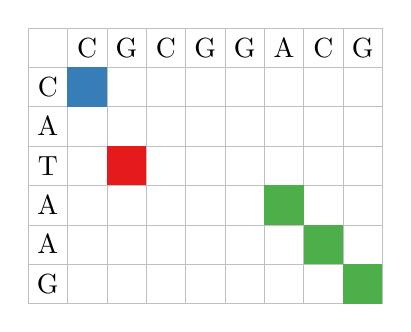
\begin{tikzpicture}[box/.style={rectangle, fill=gray!50, minimum size=0.5cm}]
\draw[very thin, color = gray!50, step = 0.5] (0,0) grid (4.5, 3.5);
\node at (0.25,2.75) {C};
\node at (0.25,2.25) {A};
\node at (0.25,1.75) {T};
\node at (0.25,1.25) {A};
\node at (0.25,0.75) {A};
\node at (0.25,0.25) {G};
\node at (0.75,3.25) {C};
\node at (1.25,3.25) {G};
\node at (1.75,3.25) {C};
\node at (2.25,3.25) {G};
\node at (2.75,3.25) {G};
\node at (3.25,3.25) {A};
\node at (3.75,3.25) {C};
\node at (4.25,3.25) {G};
\node[box, fill=colorB] at (0.75, 2.75){};
\node[box, fill=colorR] at (1.25, 1.75){};
\node[box, fill=colorG] at (3.25, 1.25){};
\node[box, fill=colorG] at (3.75, 0.75){};
\node[box, fill=colorG] at (4.25, 0.25){};
% \matrix [draw, below right, draw=none] at (current bounding box.north east) {
%         % \node[box, fill=viridis0, scale=0.75] {0\%}; \\
%         \node[box, fill=viridis1, scale=0.75] {00-09\%}; \\
%         \node[box, fill=viridis2, scale=0.75] {10-19\%}; \\
%         \node[box, fill=viridis3, scale=0.75] {20-29\%}; \\
%         \node[box, fill=viridis4, scale=0.75] {30-29\%}; \\
%         \node[box, fill=viridis5, scale=0.75] {\textcolor{white}{40-49\%}}; \\
%         \node[box, fill=viridis6, scale=0.75] {\textcolor{white}{50-59\%}}; \\
%         \node[box, fill=viridis7, scale=0.75] {\textcolor{white}{60-69\%}}; \\
%         \node[box, fill=viridis8, scale=0.75] {\textcolor{white}{70-79\%}}; \\
%         \node[box, fill=viridis9, scale=0.75] {\textcolor{white}{80-89\%}}; \\
%         \node[box, fill=viridis10, scale=0.75] {\textcolor{white}{90-100\%}}; \\
%     };
\end{tikzpicture}
